\section{Experimental setup and procedure} 
\label{sec:setup}

The experiment is conducted as described in the manual \cite{Anleitung47} with the setup shown in figure \ref{fig:setup}. \newline
The copper sample is placed inside the recipient that is first evacuated and then filled with helium gas at atmospheric pressure.
To cool the sample, the recipient is placed inside a Dewar surrounding it with liquid nitrogen.
The temperature is measured using a PT-100 resistor that measures the temperature using the dependence of resistance on temperature.
After the sample has reached a temperature of about \SI{80}{\kelvin}, the vacuum pump is turned on again reduce the internal pressure to as low as possible to reduce heat loss to convection.
Next, the sample is heated by a heating coil that is controlled by a power supply. 
The temperature of the sample is again measured using a PT-100 resistor and can be calculated via 
\begin{align}
    T = 0.00134 \cdot R^2 + 2.296 \cdot R + 4.095,
    \label{eq:temp}
\end{align}
To further reduce the heat loss, the sample is surrounded by a radiation shield.


\begin{figure}[H]
	\centering
    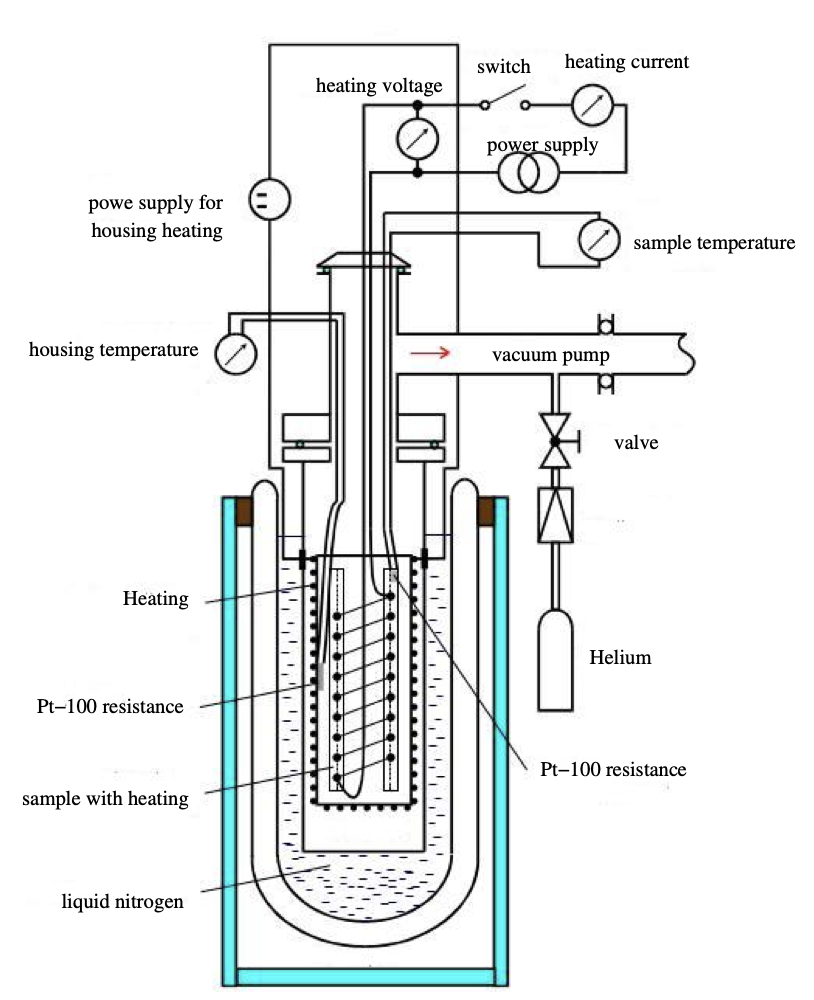
\includegraphics[width=0.6\linewidth]{data/experimental_setup.png}
	\caption{Schematic drawing of the experiment setup \cite{Anleitung47}.}
	\label{fig:setup}
\end{figure}